\documentclass[12pt,german]{article}

\usepackage[left=2cm, right=2cm, top=2cm, bottom=3.5cm, landscape=false]{geometry}

\usepackage{graphicx}
\usepackage{float}

\usepackage{tabularx}
\newcolumntype{R}{>{\raggedleft\arraybackslash}X}
\newcolumntype{L}{>{\raggedright\arraybackslash}X}
\newcolumntype{C}{>{\centering\arraybackslash}X}
\usepackage{booktabs}
\usepackage{dcolumn}

\usepackage[ngerman]{babel}

\usepackage{amsmath}

\title{\vspace{-1.5cm}Protokoll Gammaspektrometrie}
\author{Fuchs, Gutmann, Kosbab, Kowal, Steindorf, Fälker, Richter}
\setlength\parindent{0pt}


\begin{document}
    \maketitle
    \tableofcontents

    \section{Kurzbeschreibung des Versuches}
    \begin{itemize}
        \item Mithilfe von Cobalt-60 werden die Detektoren kalibriert, die Kalibrierung wird mit Cäsium-137 validiert.
        \item Auf Millimeterpapier wird die Linearität der Zuordnung von Kanallage zu Energie nachgewiesen.
        \item Es wird eine Kupfer-Probe für 10 Minuten aktiviert, anschließend mit dem Detektor ausgewertet und 10 Minuten später erneut ausgewertet.
        \item Im Reaktor wird die unbekannte Probe für 10 Minuten aktiviert.
        \item Die unbekannte Probe wird anhand der Fotopeaks ausgewertet, aufgrund verschobener Kalibrierung wird sie jedoch gegen eine neue unbekannte Probe ausgetauscht.
        \item Die neue Probe wird anhand der Fotopeaks identifiziert.
    \end{itemize}
    \newpage

    \section[Vergleich der Auflösung zwischen Halbleiter-Detektor und Szintillator]{Vergleich der Auflösung zwischen Halbleiter-Detektor und Szintillator am Beispiel von Cobalt-60}
    \begin{figure}[H]
        \begin{minipage}[t]{0.475\textwidth}
            \centering
            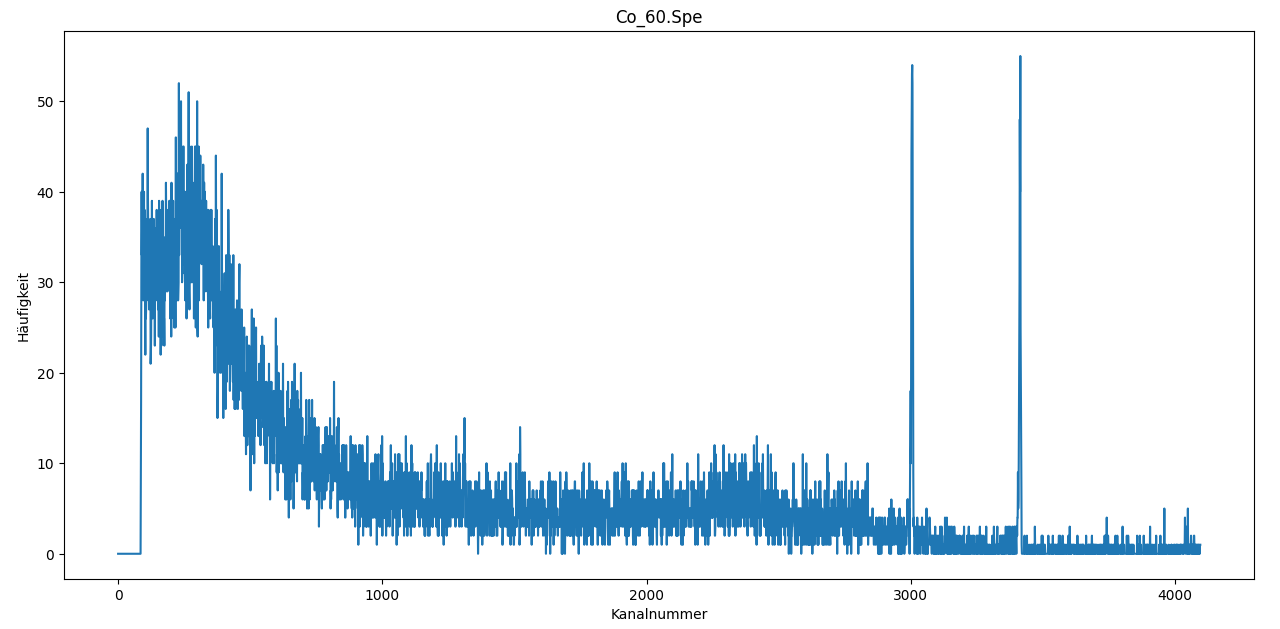
\includegraphics[width=1\textwidth]{pics/Co_60.png}
            \caption{Ge(Li) - Halbleiterdetektor}
        \end{minipage}
        \hfill
        \begin{minipage}[t]{0.475\textwidth}
            \centering
            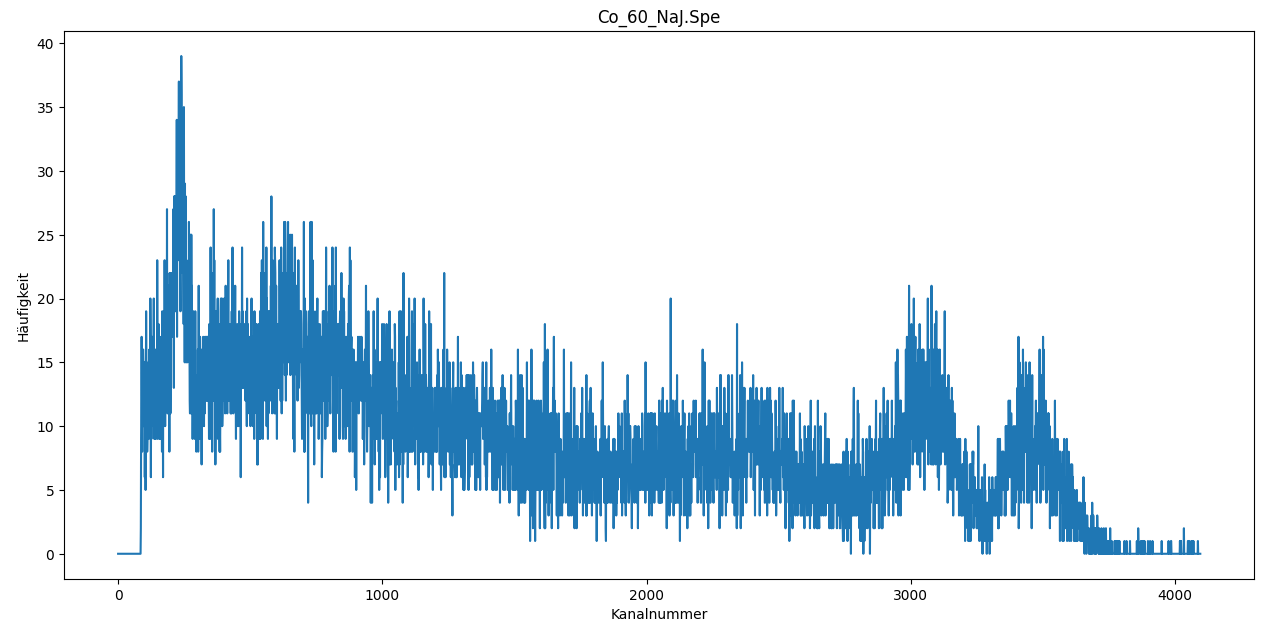
\includegraphics[width=1\textwidth]{pics/Co_60_NaJ.png}
            \caption{NaJ(TI) - Szintillator}
        \end{minipage}
    \end{figure}
    Es ist erkennbar, dass die Auflösung des Halbleiterdetektors höher ist als die des NaJ-Szintillators.
    Die Halbwertsbreite eines Peaks beträgt im NaJ-Szintillator ca. 200 Kanäle, im Halbleiterdetektor beträgt sie ca. 10 Kanäle.

    \section{Energiekalibrierung des Spektrometers mit Ge(Li)-Detektor}
    \begin{figure}[H]
        \centering
        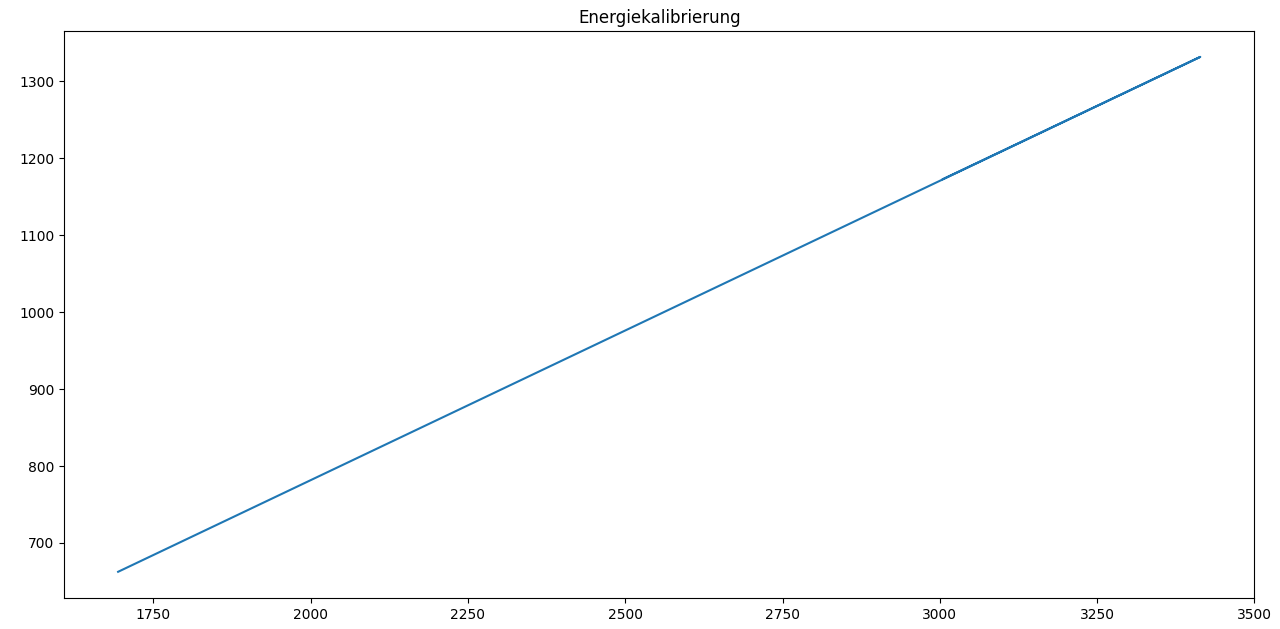
\includegraphics[width=0.7\textwidth]{pics/energiekalibrierung.png}
        \caption{Zusammenhang zwischen Kanallage und Energie}
        \label{fig:kanalenergie}
    \end{figure}
    Es werden die Kanallagen und Energien von Cobalt-60 und Cäsium-137 in einem Diagramm aufgetragen.
    Wie in Abbildung \ref{fig:kanalenergie} zu sehen, besteht zwischen Kanallage und  Energie des Fotopeaks ein linearer Zusammenhang.

    \section{Auswertung von Kupfer}
    \begin{table}[H]
        \begin{tabularx}{\textwidth}{L|R|R|R|R}
            \toprule
            \centering \textbf{Abklingzeit} & \centering\textbf{Messzeit $[s]$} & \multicolumn{2}{c|}{\textbf{Netto-Peakflächen $[\#\, Impulse]$}} & \multicolumn{1}{c}{\textbf{Peakflächen-}} \\
            \centering \textbf{$[min]$} & & \centering Cu-66 & \centering Cu-64 & \multicolumn{1}{c}{\textbf{verhältnis}} \\
            \midrule
            $0$ & $200$ & $625$ & $3073.5$ & $4.9176$ \\
            $10$ & $200$ & $126$ & $2855.5$ & $22.6627$ \\
            \bottomrule
        \end{tabularx}
    \end{table}



    \section{Identifizierung einer unbekannten Probe}
    Nach 10-minütiger Aktivierung der unbekannten Probe wird mithilfe des Ge(Li)-Halbleiterdetektors ihr Gammaspektrum gemessen. Es ergibt sich folgende graphische Auswertung: \\
    \begin{figure}[H]
        \centering
        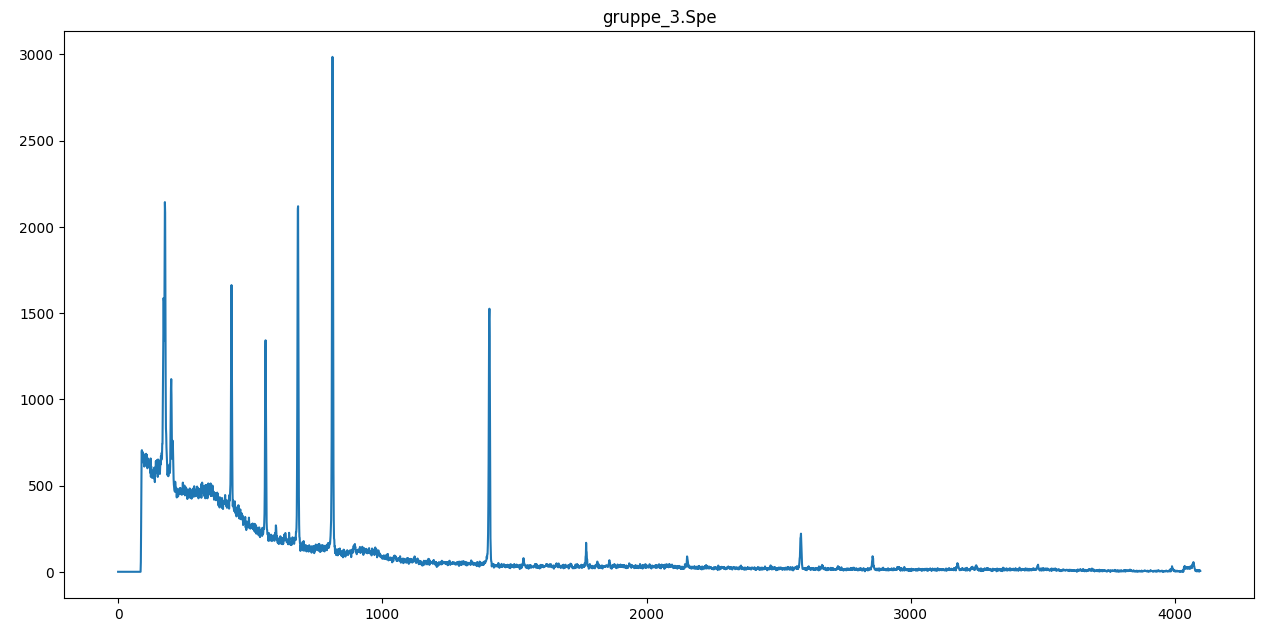
\includegraphics[width=1.0\textwidth]{pics/gruppe_3.png}
        \caption{Gammaspektrum der unbekannten Probe}
    \end{figure}

    Anschließend kann je nach gewünschter Genauigkeit eine visuelle oder rechnerische Peakbestimmung durchgeführt werden. \\
    Als rechnerische Peakanalyse wurde im Zuge dieses Protokolls die vom Analyseprogramm erstellte SPE-Datei eingelesen sowie mithilfe eines Vergleichs der Anstiege benachbarter Abschnitte die Peakkandidaten aufgestellt. \\
    Anschließend wurden durch Vergleich mit je 20 Umgebungskanälen sowie diverser Mindestanforderungen an die Peakhöhe eine feinere Auswahl möglicher Fotopeaks herausgefiltert. \\
    Diese Analyse lieferte folgende Kandidaten für Fotopeaks: \\
    \begin{figure}[H]
        \centering
        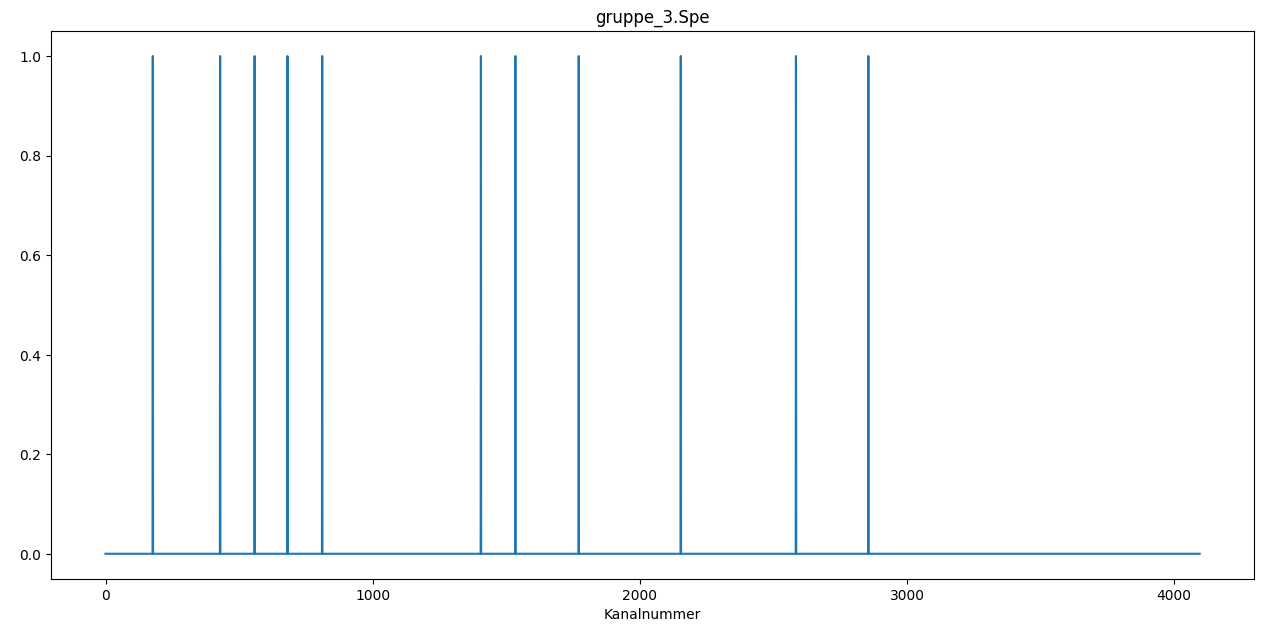
\includegraphics[width=1.0\textwidth]{pics/gruppe_3_peaks.png}
        \caption{Kandidation für Fotopeaks}
    \end{figure}
    
    Mithilfe während des Versuches mitgeschriebener, nach Kalibrierung erzeugter Kanalnummer-Energie-Paaren, kann anschließend mittels lineare Regression (siehe Abbildung \ref{fig:kanalenergie}) näherungsweise die Energiekalibrierung des Analyseprogramm rekonstruiert werden. \\
    
    \begin{table}[H]
        \centering
        \begin{tabularx}{0.5\textwidth}{R|R}
            \toprule
            \textbf{Kanalnummer} & \textbf{Energie}\([keV]\) \\
            \midrule
            428 & 186 \\
            559 & 243 \\
            679 & 295 \\
            810 & 352 \\
            1406 & 610 \\
            \bottomrule
        \end{tabularx}
        \caption{Kalibrierungspaare}
    \end{table}
    \begin{align}
        E = f(K) = 0.43345 K + 0.66809
    \end{align}
    
    Damit können nun den errechneten Fotopeaks die jeweiligen Energien bezüglich der im Praktikumsversuch verwendeten Kalibrierung zugeordnet werden: \\

    \begin{table}[H]
        \centering
        \begin{tabularx}{0.5\textwidth}{R|R}
            \toprule
            \textbf{Kanalnummer} & \textbf{Energie \([keV]\)} \\
            \midrule
            177 &  77.39 \\
            429 & 186.62 \\
            558 & 242.53 \\
            681 & 295.85 \\
            811 & 352.20 \\
            1405 & 609.67 \\
            1534 & 665.58 \\
            1771 & 768.31 \\
            2153 & 933.89 \\
            2584 & 1120.70 \\
            2855 & 1238.17 \\
            \bottomrule
        \end{tabularx}
        \caption{durch Kalibrierung gegegbene Relation zwischen Kanalnummer und Energie}
    \end{table}

    Die gemessenen Fotopeaks können nun mit den Gammaenergien bekannter Nuklide verglichen werden, um eine Identifizierung der unbekannten Probe zu erreichen. \\
    Der bei einer Energie von \(77.39\, keV\) identifizierte Peakkandidat stellt sich bei Vergrößerung des Spektrums als eine Ansammlung mehrerer Impulsausschläge heraus: \\
    
    \begin{figure}[H]
        \centering
        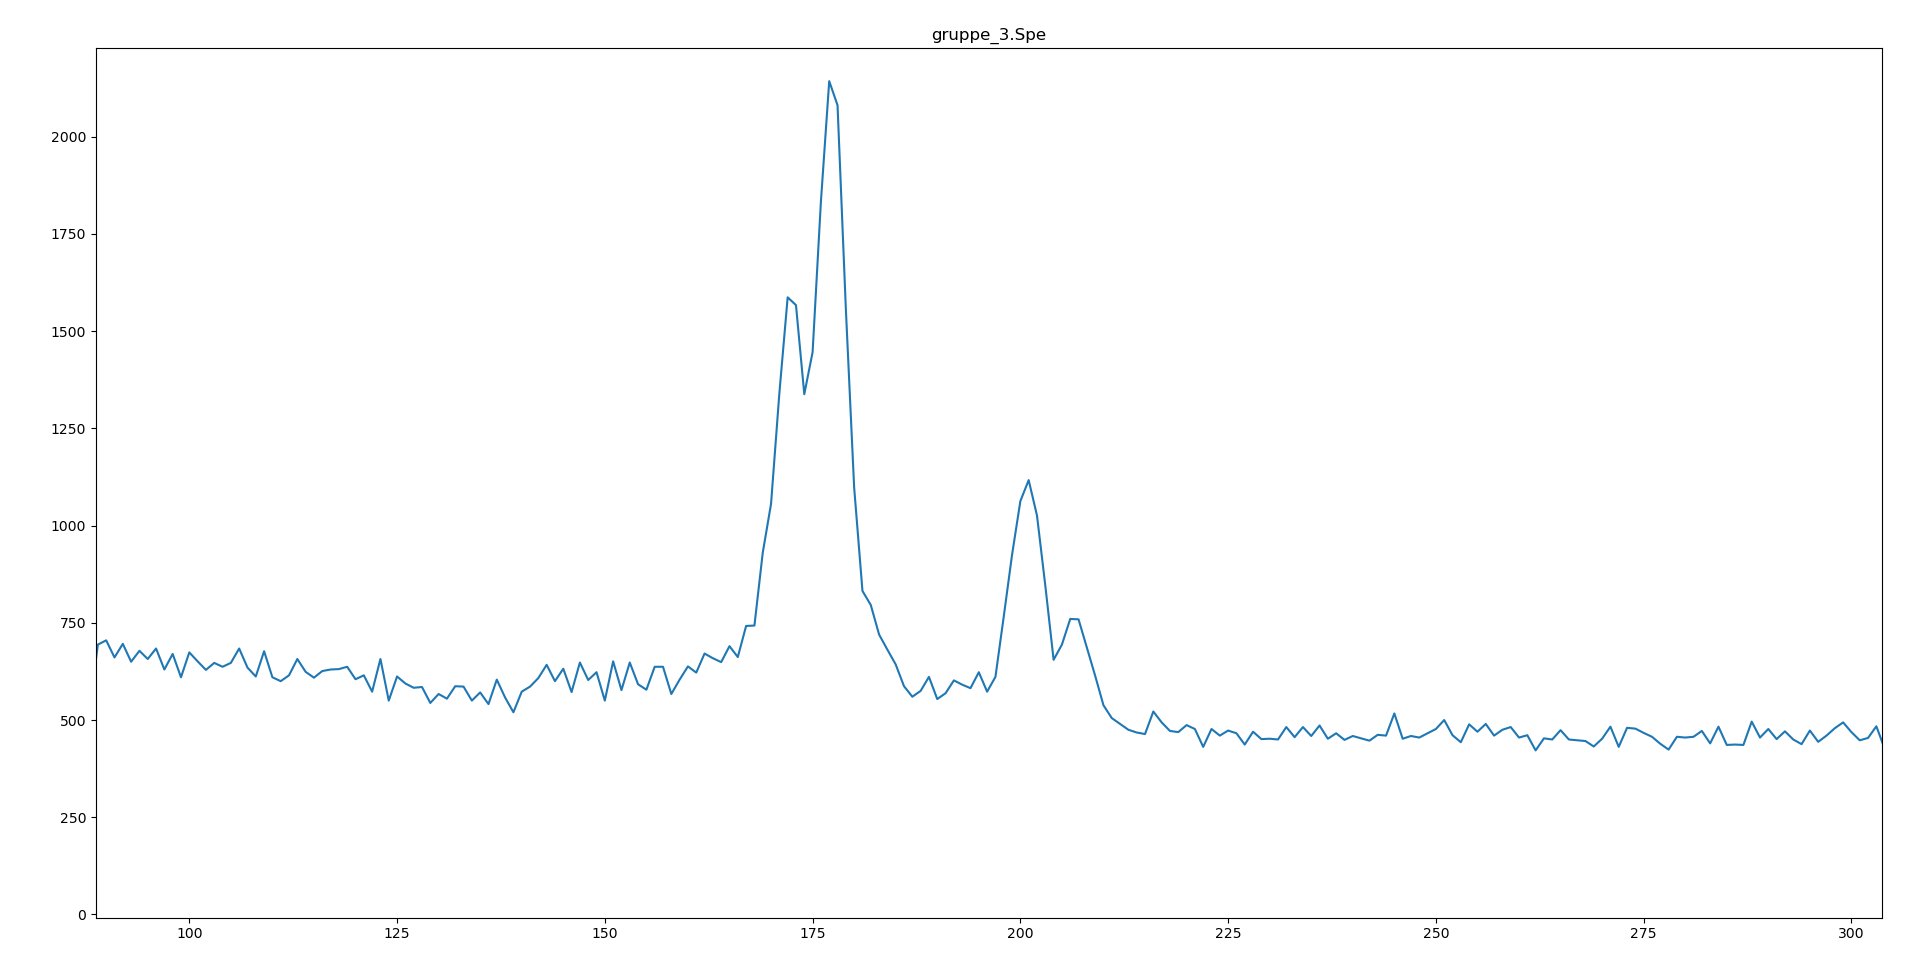
\includegraphics[width=1.0\textwidth]{pics/gruppe_3_xrays.png}
        \caption{Vergrößerung des Gammaspektrums der unbekannten Probe um 77.39 keV}
    \end{figure}

    Aufgrund dieser diffusen Verteilung sowie der Lage im Energiespektrum lässt sich hinter diesen Impulsen Röntgenstrahlung vermuten. \\
    Alle Peakkandidaten oberhalb der Kanalnummer 1500 haben aufgrund ihrer geringen Peakhöhe vermutlich ebenfalls keinen direkten Ursprung im Gammazerfall des Ausgangselements, sondern werden von Zerfallsprodukten emittiert. \\
    Damit ergeben sich für die Recherche Fotopeaks mit Energien im Bereich von 186.5 keV, 242.5 keV, 296 keV, 352 keV sowie 609.5 keV. \\
    Bei der unbekannten Probe handelt es sich um Radium-Leuchtfarbe. \\
    Der Gammazerfall des zugehörigen Isotops \(^{226}\)Ra erzeugt jedoch nur für eine Energie von 186.211 keV messbare Fotopeaks. Die drei darauffolgenden Peakkandidaten werden von dem Zerfallsprodukt Blei \(^{214}\)Pb, sowie alle weiteren von dem Zerfallsprodukt Bismut \(^{214}\)Bi erzeugt. \\
    Aus diesem Grund ist es während des Praktikumsversuches nicht gelungen, eine eindeutige Identifizierung der unbekannten Probe anhand des gemessenen Gammaspektrums zu erreichen. 
    \begin{table}[H]
        \centering
        \begin{tabularx}{1.0\textwidth}{R|R|R|R}
            \toprule
            Nuklid &  Messwert \([keV]\) & Literaturwert \([keV]\) & Abweichung \([keV]\) \\
            \midrule
            \(^{226}\)Ra & 186.62 & 186.211 &   0.41 \\
            \(^{214}\)Pb & 242.53 & 241.997 &   0.54 \\
            \(^{214}\)Pb & 295.85 & 295.224 &   0.62 \\
            \(^{214}\)Pb & 352.20 & 351.932 &   0.26 \\
            \(^{214}\)Bi & 609.67 & 609.312 &   0.35 \\
            \(^{214}\)Bi & 665.58 & 665.453 &   0.13 \\
            \(^{214}\)Bi & 768.31 & 768.356 &   0.05 \\
            \(^{214}\)Bi & 933.89 & 934.061 &   0.18 \\
            \(^{214}\)Bi & 1120.70 & 1120.287 &   0.42 \\
            \(^{214}\)Bi & 1238.17 & 1238.110 &   0.06 \\
            \bottomrule
        \end{tabularx}
        \caption{Vergleich gemessener zu tatsächlicher Energiewerte}
    \end{table}
    Die Energien der gemessenen Peakpositionen ensprechen dabei sehr exakt den tatächlichen Gammastrahlungsenergien der Zerfallsprodukte, es ergibt sich eine maximale Abweichung von 0.62354 keV sowie eine durchschnittliche Abweichung von 0.300839 keV.

\end{document}